\chapter {Evaluation}
We now evaluate the effectiveness of \pbox, \phub, \plink and \cmpi in their perspective environments in accelerating distributed training workloads.

\section{Effectiveness of \phub and \pbox}
We added support for \phub{}'s API to MxNet, replacing its PS. We evaluated \phub by comparing it to MxNet's unmodified PS. We had five goals in our evaluation: (1) to assess the impact of \phub software and the \pbox hardware on training throughput, (2) to identify the importance of each optimization, (3) to determine the limits of \pbox, (4) to evaluate effectiveness of \pbox as a rack-scale service. and (5) to demonstrate the cost-effectiveness of the \phub.


\subsection{Experimental Setup}
We evaluated our system with 8 worker nodes and one specially configured \pbox node. The workers were dual socket Broadwell Xeon E5-2680 v4 systems 
% with 28 cores at 2.4 GHz -- we can omit details as product model implies clockspeed etc to save some space.
and 64 GB of memory using 8 dual-rank DDR-2400 DIMMs. Each worker had a GTX 1080 Ti GPU % with 11 GBs of memory 
and one Mellanox ConnectX-3 InfiniBand card with 56 Gbps bandwidth in the same NUMA domain. The \pbox machine was a dual socket Broadwell Xeon E5-2690 v4 system with 28 cores % running at 2.6 GHz 
and 128 GBs of memory using 8 dual-rank DDR-2400 DIMMs. \pbox had 10 Mellanox ConnectX-3 InfiniBand cards, with 5 connected to each socket. Hyperthreading was disabled. Machines were connected with a Mellanox SX6025 56 Gbps 36-port switch.

The machines ran CentOS 7.3 with CUDA 8 and CuDNN 7 installed. Our modifications to MxNet and its PS (PS-Lite) were based on commit 2ce8b9a of the master branch in the PS-Lite repo. We built MxNet with GCC 4.8 and configured it to use OpenBLAS and enable SSE, the Distributed Key Value Store, the MxNet Profiler, and OpenMP. We used Jemalloc, as suggested by MxNet.

\subsection{DNNs Used in the Evaluation}
We evaluated \phub{}'s performance by training state-of-the-art deep neural networks using reference code provided with MxNet. %While we did not modify the code, 
%We adjusted layer count, per worker batch size, and the number of workers and servers to launch. 
We implemented a cache-enabled optimizer using SGD with Nesterov's accelerated gradient method \cite{nesterov1983method} and a cache-enabled aggregator for \phub{}. We chose a per GPU batch size of 32 when possible; for ResNet 269 and ResNext 269, we used 16 and 8, respectively, since 32 did not fit in the GPU. We did not use MXNet's GPU memory optimizations~\cite{chen2016training} because they slow down training.

\begin{table}[t!]
	\centering
	\footnotesize
	\begin{tabular}{|c|c|c|c|}
		\hline 
		Name (Abbr)           & Model Size & Time/batch & Batch \\
		\hline
		AlexNet (AN)      & 194MB & 16ms &  32 \\
		\hline 
		VGG 11 (V11)       & 505MB & 121ms & 32 \\
		\hline
		VGG 19 (V19)      & 548MB & 268ms & 32 \\
		\hline
		GoogleNet (GN)   &  38MB & 100ms & 32 \\
		\hline
		Inception V3 (I3) & 91MB  & 225ms & 32 \\
		\hline
		ResNet 18 (RN18)   & 45MB & 54ms & 32 \\
		\hline
		ResNet 50 (RN50)   & 97MB & 161ms & 32 \\
		\hline  
		ResNet 269 (RN269)  & 390MB & 350ms & 16 \\
		\hline
		ResNext 269 (RX269) & 390MB & 386ms & 8 \\
		\hline
	\end{tabular}
	\caption{Neural networks used in our evaluation. Time/batch refers to the forward and backward compute times for a batch.}
	\label{table:networkCharacterization}
\end{table}


Table \ref{table:networkCharacterization} summarizes the neural networks used in our evaluation, which include both winners of the ImageNet challenge and other recent, popular networks. We used the reported model size from MxNet and measured the forward and backward passes time on a single GPU. % with the batch sizes described previously. %We turned off aggregation and optimization for this measurement; therefore, the time represents only that for forward and backward passes.

We report only training throughput in our evaluation since our modifications did not change accuracy: they did not change the computations that were performed. We trained multiple DNNs to convergence to verify this.



\subsection{Training Performance Evaluation}
%We explored training performance using \phub, normalized to unmodified MxNet's performance. 
We include multiple results to highlight the effects of different software and hardware optimizations on \phub{}'s training performance. We measured training performance by comparing the total time of 200 iterations. We used two IB network configurations. This lets us compare training performance for two different compute/bandwidth ratios: (1) where GPUs were much faster than the network, and (2) with ample network bandwidth resources. In both setups, we used 8 workers.
%Both results reflect the benefit of an optimized gradient processing pipeline from the \phub software stack and the benefit of using hardware with balanced resources (\pbox). %\TODO{DO WE NEED 56Gbps IT LOOKS BAD WITH NEW BASELINE.}

\begin{figure}[t!]
    \centering
	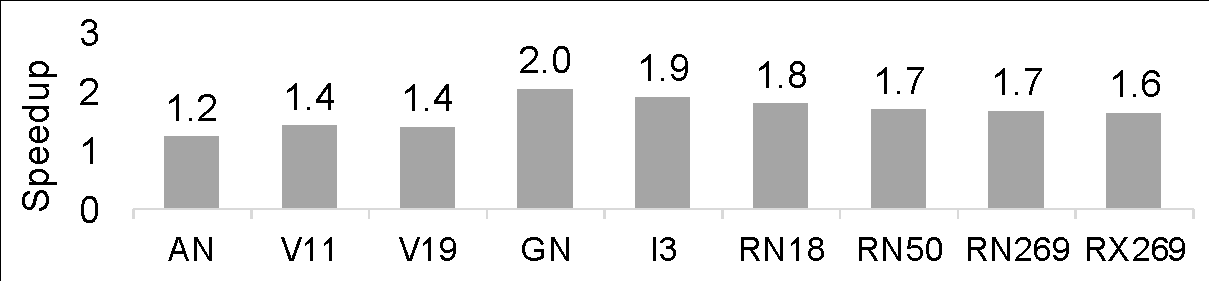
\includegraphics[width=.7\linewidth,trim=8 4 4 4,clip]{Figures/IBBenefits.pdf}
	\caption{Speedup from a faster data plane that supports zero copy.}
	\label{fig:IBBenefits}
\end{figure}

\subsubsection{Benefit of a Faster Data Plane}
Figure \ref{fig:IBBenefits} shows the performance of replacing the communication stack of the MxNet PS with a native InfiniBand implementation (MxNet) that had all optimizations enabled. This lets us see the benefit of switching to an optimized network stack without changing the PS architecture. %We believe similar speedup can be observed on a RoCE-based implementation, because the benefit comes mainly from zero copy. 
We used our \textit{enhanced baseline MxNet} in all the following evaluation.

\subsubsection{Other Software and Hardware Optimizations}
We now quantify further benefits from \phub{}'s software and hardware optimizations. 
We used CS MxNet in this comparison.
\pshard{} results were obtained by running \phub software on each worker as CS PSs. \pbox results represent running \phub software on our single \pbox machine as a NCC PS. We omit results for NCS and CC PSs for clarity. They performed similarly to \pbox results.




% placed here to be on same page as text
\begin{figure*}[t!]
	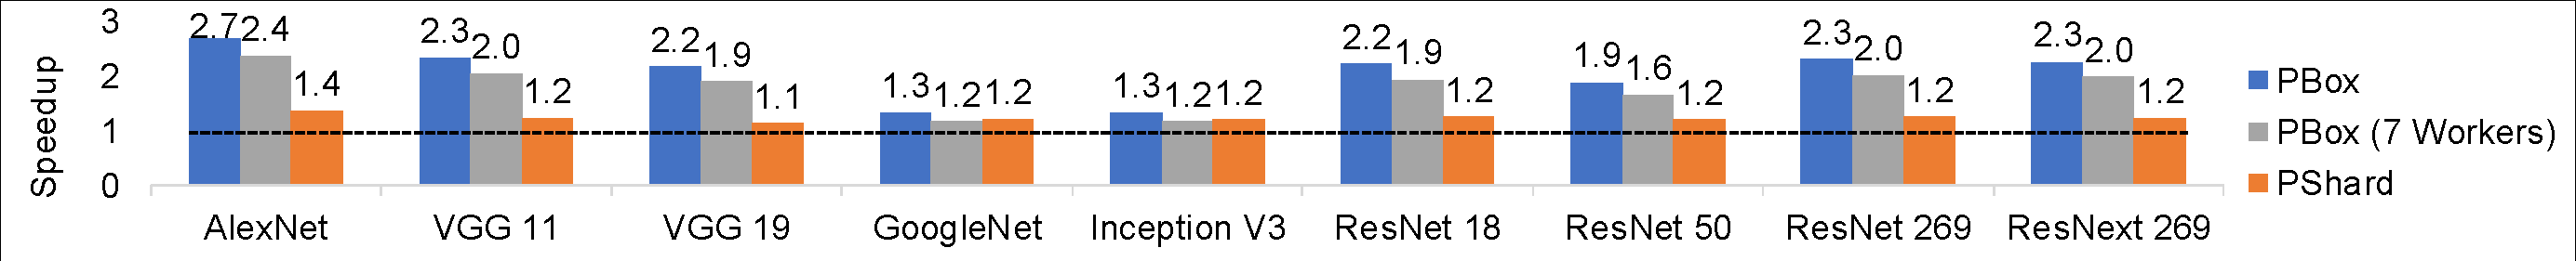
\includegraphics[width=\linewidth,trim=4 4 4 4,clip]{Figures/8GbpsRealTraining_SOCC.pdf}
	\caption{Training performance on a cloud-like 10 Gbps network. Results are normalized to sharded MxNet (\textit{enhanced baseline}).}
	\label{fig:real-8gb}
\end{figure*}

% placed here to be on same page as text
\begin{figure}[t!]
    \centering
	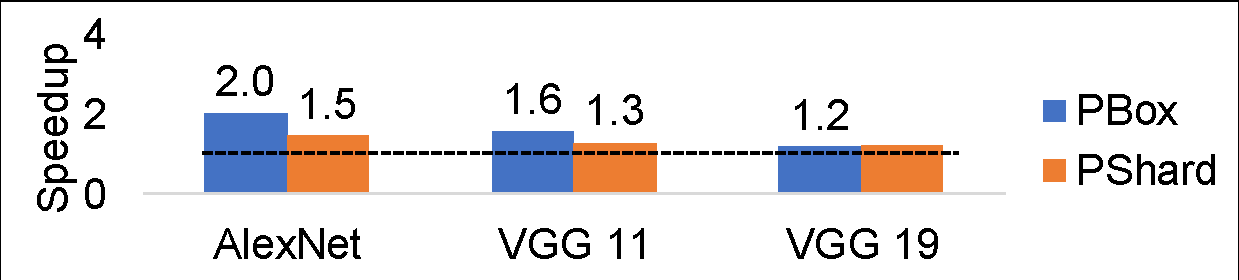
\includegraphics[width=.5\linewidth,trim=8 4 4 4,clip]{Figures/56GbpsRealTraining_SOCC.pdf}
	\caption{Training performance on a 56 Gbps network compared to MxNet (\textit{enhanced baseline}). Computation speed bottlenecked training throughput for all but AlexNet and VGG.}
	\label{fig:real-56gb}
\end{figure}

\begin{figure}
    \centering
	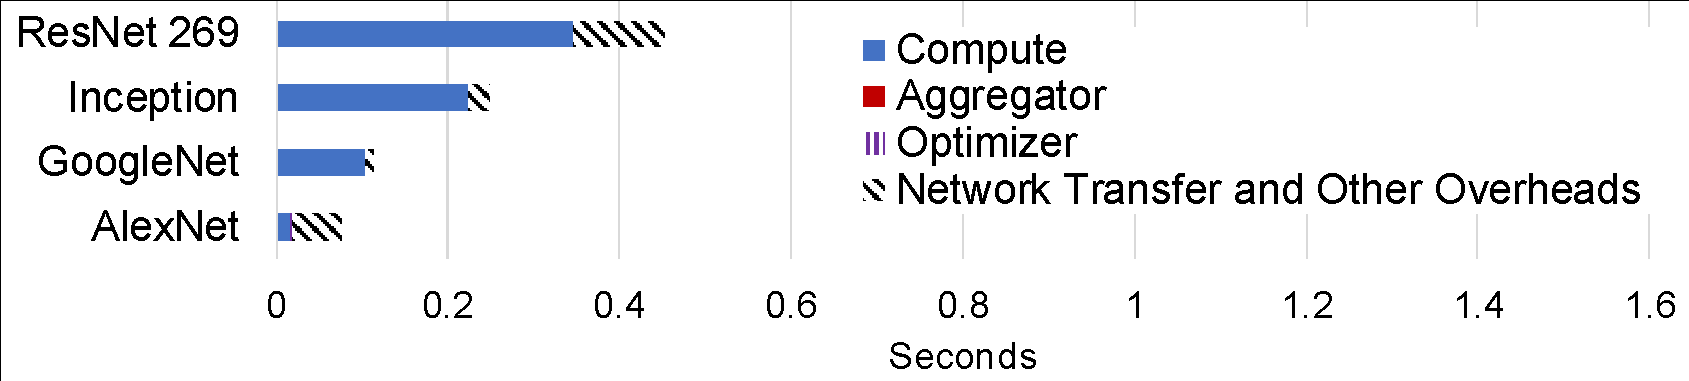
\includegraphics[width=.7\linewidth,trim=4 2 2 4,clip]{Figures/PHubOverheadBreakdown.pdf}
	\caption{Progressive overhead breakdown of \phub. Compared to Figure~\ref{fig:overheadBreakdown}, GPU compute time now dominates training time. Aggregator and optimizer have minimum overhead, and are barely visible.}
	\label{fig:phubOverheadBreakdown}
\end{figure}

Figure~\ref{fig:real-8gb} shows training performance on a cloud-like 10 Gbps network, obtained by down-clocking our IB links. In this configuration, the ratio of GPU batch execution time to network serialization delays is such that the reduced communication and faster aggregation of \pbox significantly affects runtime. In addition, we provide speedup when training with only 7 workers and \pbox, \textit{so that the total machine count in the system is equal to the baseline}.

Figure~\ref{fig:real-56gb} shows training performance on 56 Gbps InfiniBand.
%% In this setup, training throughput of networks such as GoogleNet, Inception, ResNet, and ResNext is limited by speed of forward and backward passes, the time to execute forward and backward passes exceeds that of parameter exchange; thus, raising network bandwidth only marginally affects the total throughput of \phub versus MxNet.
In this setup, for networks such as GoogleNet, Inception, ResNet, and ResNext, forward and backward pass execution time limits training throughput; thus, raising network bandwidth only marginally affects the total throughput of \pbox versus MxNet. Since \phub never slows down training, we omit results of these networks (1x speedup) for clarity. We expect larger speedups with newer, faster GPUs such as the NVidia V100, for these networks. Significant speedup is still achieved with models that have large communication-to-computation ratios, such as AlexNet and VGG; these models remained network-bound even on 56 Gbps links.

%In both cases, the gap between \pbox and \pshard highlights the benefits of non-colocated servers: \textit{they roughly halve the per link bandwidth usage, which makes a significant performance difference in the cloud}. 
The gap between \pshard and MxNet signifies the benefit of software optimizations. The gap between \pshard and \pbox highlights both the benefit of a non-colocated server that \textit{halves the per link bandwidth usage, yielding a significant performance difference}, and the benefit of the hardware optimizations.

%The gap between \pshard and MxNet shows the benefit of \phub software stack optimizations (\mysection\ref{sec:commonOptimizations}), and the gap between MxNet and the baseline reflects the effectiveness of an optimized communication stack (\mysection\ref{sec:IBOptimization}). %\TODO{more explanation}

%Figure~\ref{fig:real-2gb} shows an unbalanced condition where the provisioned compute resource is significantly faster than network bandwidth. We achieved this by reducing our network bandwidth to 2 Gbps; this lets us model the performance of 28x faster GPUs with our 56 Gbps network. Although the baseline parameter servers are more than capable of processing messages at this network speed, the workers' network bandwidth is highly contended by its colocated parameter server instance during parameter synchronization. \phub achieves up to 3x speedup over sharded PSLite-ZMQ by avoiding this worker/shard contention, and providing faster aggregation and optimization.

Figure \ref{fig:phubOverheadBreakdown} breaks down the overhead in different distributed training stages when running \phub in the same setup as Figure \ref{fig:overheadBreakdown}. Compared to Figure \ref{fig:overheadBreakdown}, \textit{\phub reduces overheads from data copy, aggregation, optimization, and synchronization, and fully overlaps these stages, shifting the training back to a compute-bound workload.}


\subsection{Performance with Infinitely Fast Compute}
We used a benchmark to assess the efficiency of \phub{}'s gradient processing pipeline to avoid being bottlenecked by our workers' GPUs. We implemented a special MxNet engine, called \code{ZeroComputeEngine}, based on the original \code{ThreadedEnginePerDevice}, which replaces training operators (such as convolution) with an empty routine. Only the synchronization operators (\code{WaitForVar}, \code{KVStoreDistPush} and \code{KVStoreDistPull}) are actually executed. This engine effectively simulates arbitrarily fast forward and backward passes on the worker side, pushing the limits of \phub.

We used ResNet 18 as the test network. We measured how fast each worker can run in this setup individually with the \pbox, then gradually added more workers to plot total system throughput.

%By spreading the communication equally on the 10 interfaces on the \pbox and utilizing all processors, a worker can perform 110 iterations per second, producing 10GB/s of bidirectional throughput. A single \phub core is enough to saturate a worker. Aggregation and optimization are disabled for this benchmark. We set our "training batch size" to 1 for this benchmark so we measure only the parameter exchange rate. 

Figure \ref{fig:FakeTrainingWithAggOpt} shows the results of running the benchmark with \pbox, \pshard and multiple baseline configurations. \pbox  provided linear scaling with 8 workers and outperformed the baseline by a large margin (up to 40x). \pbox had 2x the speedup of \pshard{} because each of its interfaces needed to move only about half the amount of data compared to colocated servers.

\begin{figure}[t!]
    \centering
	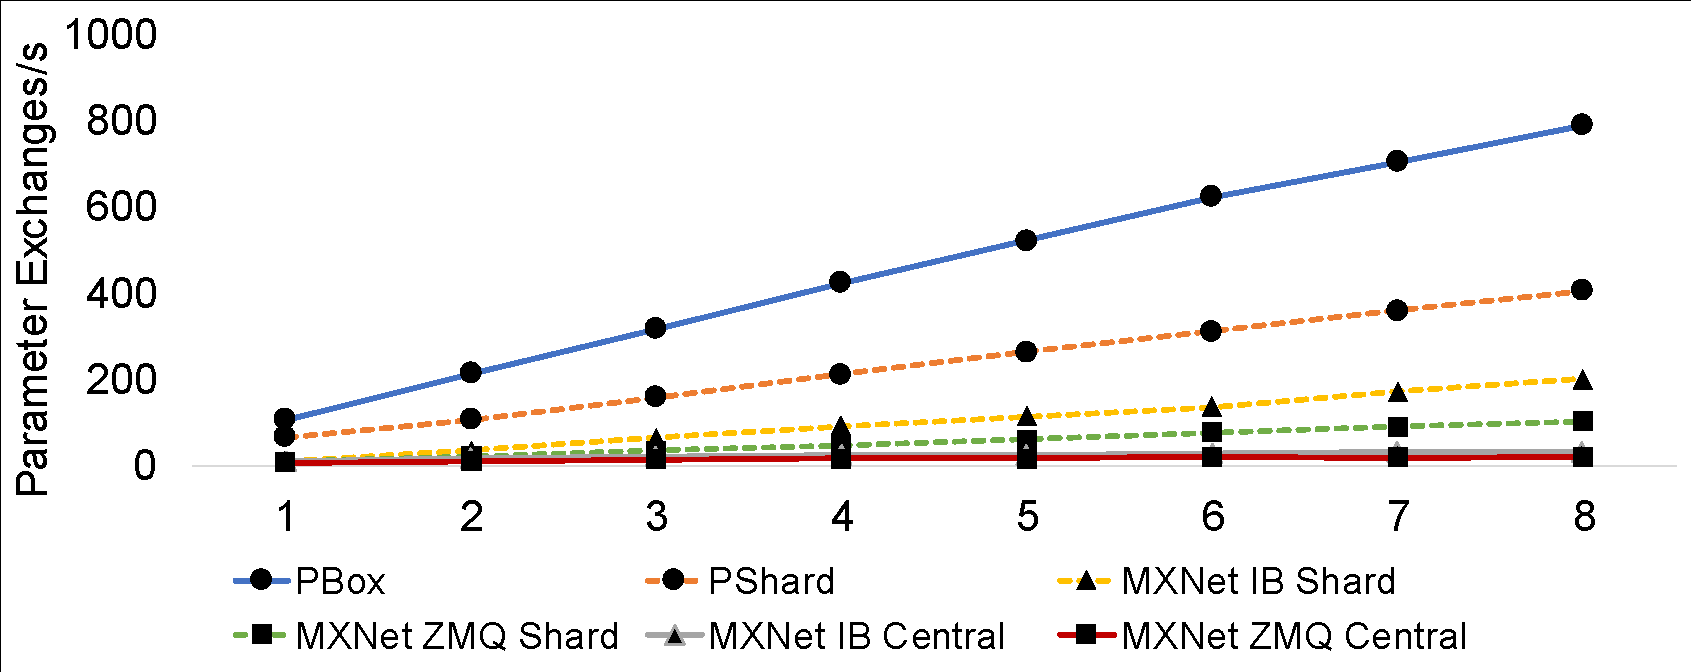
\includegraphics[width=.7\linewidth,trim=3 1 1 3,clip]{Figures/FakeTrainingWithAggOpt.pdf}
	\caption{\pbox provides linear scaling of throughput for 8 worker nodes with infinitely fast compute, training ResNet 18.}
	\label{fig:FakeTrainingWithAggOpt}
\end{figure}


\subsection{Exploiting Locality}
\label{sec:locality}
To postpone hitting the memory bandwidth limit, it is crucial to exploit locality in network interfaces and processor caches. This section evaluates the effectiveness of \phub{}'s key assignment scheme and tall aggregation/optimization in leveraging locality.

\vspace{0.05in}
\noindent \textbf{Key Affinity in \pbox:}
%\subsubsection{Key affinity in \pbox}
\label{sec:affinity}
We evaluate two schemes for connecting workers to \pbox to exploit locality and load balancing. In \textit{Key by Interface/Core mode}, workers partition their keys equally across different interfaces on the \pbox. This mode better utilizes cache by binding a key to a particular interface, core and a NUMA node. %, computation for that key can more effectively use cache. 
This mode also exploits locality in time as workers are likely to generate the same key close to each other in synchronous training.

In \textit{Worker by Interface mode}, each worker communicates with the server through a single interface. This lets \phub exploit locality within a single worker. It also provides naturally perfect load balancing across interfaces and cores at the cost of additional communication and synchronization for each key within the server because keys are scattered across all interfaces and sockets.

%We used the same \code{ZeroComputeEngine} to evaluate the aforementioned approaches. 
We found that Key by Interface/Core provided 1.43x (790 vs 552 exchanges/s) better performance than Worker by Interface mode with \code{ZeroComputeEngine}. The locality within each worker could not compensate for synchronization and memory movement costs.


\vspace{0.05in}
\noindent \textbf{Tall vs. Wide Parallelism:}
%\subsubsection{Tall vs. Wide Aggregation and Optimization}
%Figure \ref{fig:tallVSWide} compares throughput of \phub's tall approach to aggregation and optimization with MxNet's wide approach. 
We evaluated tall aggregation vs MxNet{}'s wide approach with ResNet 50. Tall outperformed wide by 20x in terms of performance  and provides near-perfect scaling to multiple cores. Tall aggregation benefited from increased overlap compared to wide, and wide was further hurt by the cost of synchronization.

%\begin{figure}[t!]
%	\includegraphics[width=\linewidth,trim=3 1 2 3,clip]{Figures/TallVSWide.pdf}
%	\caption{Tall aggregation/optimization was more efficient than wide aggregation/optimization.}
%	\label{fig:tallVSWide}
%\end{figure}

\vspace{0.05in}
\noindent \textbf{Caching Effectiveness in \phub:}
%\subsubsection{Caching effectiveness in \phub}
\label{eval:cache}
Caching benefits many \phub operations. For example, models can be sent directly from cache after being updated, and aggregation buffers can reside in cache near the cores doing aggregation for those keys. We now evaluate the effectiveness of caching in \phub by measuring memory bandwidth usage.

\begin{table}[t!]
	\centering
    \footnotesize
	\begin{tabular}{|c|c|c|}
		\hline 
		& Mem BW & Throughput\\
		\hline
		Opt/Agg Off & 77.5 & 72.08 \\
		\hline 
		Caching Opt/Agg & 83.5 & 71.6 \\
		\hline
		Cache-bypassed Opt/Agg & 119.7 & 40.48 \\
		\hline
	\end{tabular}
	\caption{Bidirectional memory bandwidth (GB/s) utilization in \phub when training VGG with 8 workers. The maximum memory bandwidth for the machine is 137 GB/s for read-only workloads and 120 GB/s for 1:1 read:write workloads as measured by LikWid and Intel MLC.}
	\label{table:cacheUtilizationAndAggregationOverhead}
\end{table}

Table \ref{table:cacheUtilizationAndAggregationOverhead} shows the memory bandwidth costs of communication, aggregation, and optimization on \pbox. We used 8 workers running a communication-only benchmark based on the VGG network, chosen because it had the largest model size. We first ran the benchmark with no aggregation or optimization, and we then added our two aggregation and optimization implementations.

Without aggregation and optimization, \pbox{}'s bidirectional memory bandwidth usage was stable at 77.5 GB/s. No cache was used in this case because \pbox did not touch the data (only the network interface did).

We found that the caching version of the aggregator and optimizer performed significantly better than the cache-bypassing version, which hit the maximum memory bandwidth available on the \phub machine when combined with the memory bandwidth of worker sends and receives. The caching version, on the other hand, added only 8\% to total memory bandwidth usage; aggregation and optimization added only 1\% of overhead to the overall throughput in this benchmark, fully overlapping gradient transfer. 

\begin{figure}[t!]
    \centering
	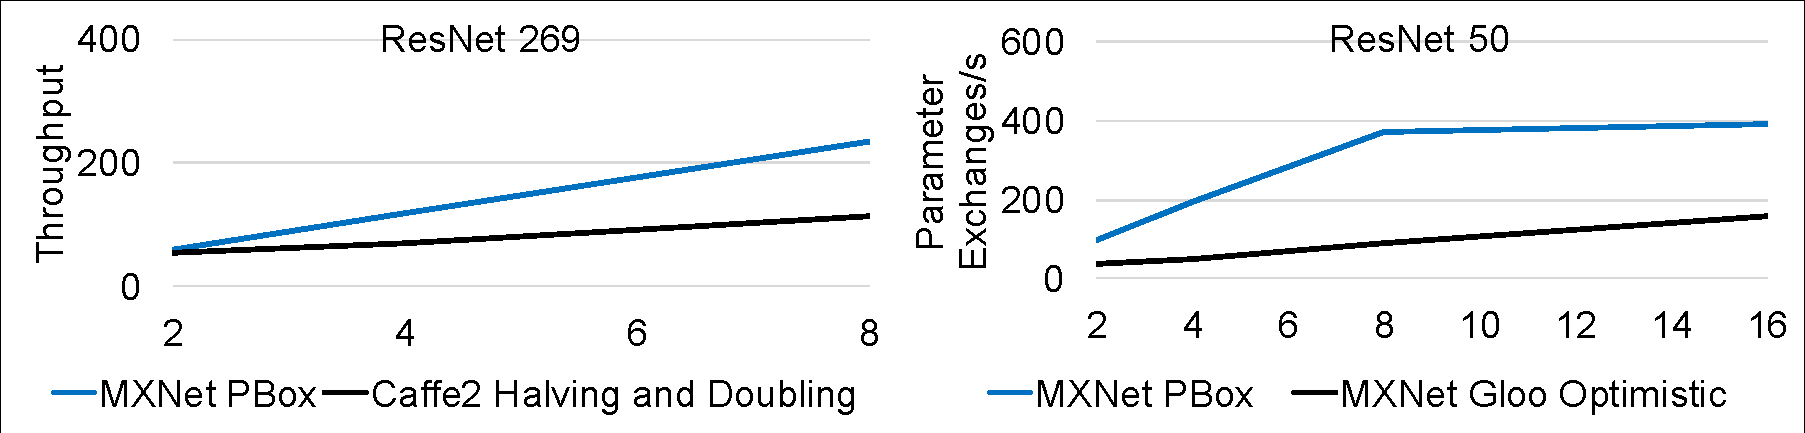
\includegraphics[width=.7\linewidth,trim=8 4 4 4,clip]{Figures/VSGloo.pdf}
	\caption{Left: Comparing Caffe2 + Gloo and MxNet + \pbox on an 10Gbps InfiniBand network. Right: Comparing MxNet + Gloo and MxNet + \pbox on a 56Gbps InfiniBand network with \code{ZeroComputeEngine}. }
	\label{fig:gloo}
\end{figure}

\vspace{0.05in}
\subsection{Comparison with Other Schemes}
%\subsection{Other Communication Schemes}
Parameter servers are not the only way to perform model updates. Frameworks such as CNTK and Caffe2 can use HPC-like approaches, such as collective communication operations~\cite{Thakur:2005:OCC:2747766.2747771, firecaffe}.

To understand how \phub compares to other communication schemes, we first ran Caffe2 and MxNet with \pbox. We used InfiniBand for both systems. We evaluated the fastest algorithm in Gloo: recursive halving and doubling, used in \cite{ImageNetIn1Hour}. Figure \ref{fig:gloo} (left) shows \pbox was nearly 2x faster. 
%This is expected because collectives, like colocated servers, cause roughly 2x traffic per link in the system, bottlenecking training performance in network bound environment.

We ported Gloo to MxNet to better assess both systems. Gloo implements blocking collective operations, but MxNet expects non-blocking operations. Therefore, we measured an optimistic upper bound by letting Gloo start aggregating the entire model as soon as the backward pass started, as if all gradients were available instantaneously. Since Gloo only does reduction, we ran our SGD/Nesterov optimizer on all nodes after reduction was complete. We used 56 Gbps IB and \code{ZeroComputeEngine} to compute bottlenecks. Figure \ref{fig:gloo} (right) shows %when given an infinitely fast compute engine and ample communication resources, 
\pbox sustained higher throughput and provided better scaling up to its limit. Two reasons account for this difference. First, collectives suffer from the same problem as colocated PSs: the interface on each participating node must process nearly 2x the data (Gloo's \code{allreduce} starts with a \code{reduce-scatter} followed by an \code{allgather}~\cite{Thakur:2005:OCC:2747766.2747771}). 
% illustrates the complexity of the scheme). 
Second, collectives frequently use multi-round communication schemes %uses multiple rounds of communication to perform reduction: 
%($logN$ rounds for $N$ workers in this case), 
whereas \pbox uses only 1 round. %, minimizing reduction latency.

% third,  \pbox moves the minimum amount of data in the network: $2MN$, where $M$ is the model size, and halving and doubling moves 

%One interesting point here is that only a fraction of the cores are required to saturate the memory bandwidth when doing aggregation and optimization. Our experiments showed that 4 cores per socket are sufficient to saturate bandwidth for these processors, but to avoid synchronization overhead in the network layer we use one core per interface (5 per socket; 10 total) for the rest of our evaluation.

%We now compare \phub's aggregator and optimizer performance with our baselines using a synthetic benchmark no-computation benchmark based on ResNet-18. Here, we add an additional baseline using MXNet with an allreduce implementation from the Gloo~\cite{Gloo,ImageNetIn1Hour} collectives library. 

%Gloo implements blocking collective operations, but MxNet expects non-blocking operations, so we provide an optimistic upper bound on aggregation performance with Gloo by allowing it to start aggregating the entire model as soon as the backward pass starts, as if the entire gradient is available instantaneously. We evaluate the two fastest algorithms in Gloo: recursive halving and doubling, which is used in \cite{ImageNetIn1Hour}, and chunked ring, which has low analytical complexity and is empirically fast in our measurement. Since Gloo only does reduction, we run our SGD/Nesterov optimizer on all nodes after reduction is complete. We include only a colocated configurations for the sharded baselines in this experiment.

%Figure \ref{fig:cacheUtilizationAndAggregationOverhead} shows the result. \phub beats sharded PSLite-ZMQ and PSLite-IB 7.6x and 3.9x, respectively,  demonstrating the efficient implementation aggregation and optimization in \phub.  \phub also beats Gloo's chunked ring and halving and doubling algorithms by 4.7x and 6.3x, respectively. This is expected since the \phub uses a single round of communication per key, per iteration, whereas for our 8 workers the collective algorithms use 7 and 3 rounds, respectively, and bandwidth is not a bottleneck in this test. We repeated this under a bandwidth limited environment (2Gbps), and found our speedup over these two collectives algorithms is 1.9x and 2.9x. In~\cite{ImageNetIn1Hour}, the halving and doubling algorithm was faster than the chunked ring, but we see the opposite result; we believe this is due to the higher implementation complexity of halving and doubling, and the lower number of workers in our cluster---too few to see the asymptotic complexity benefit. 

%Finally, \phub has a 2x advantage over PShard, which again is limited by network bandwidth due to colocation.


\subsection{Tradeoffs in Fine-Grained Key Chunking}
\label{sec:commParam}
We now examine tradeoffs in the communication layer concerning the size of key chunks and queue pair counts.

\begin{figure}[t!]
    \centering
	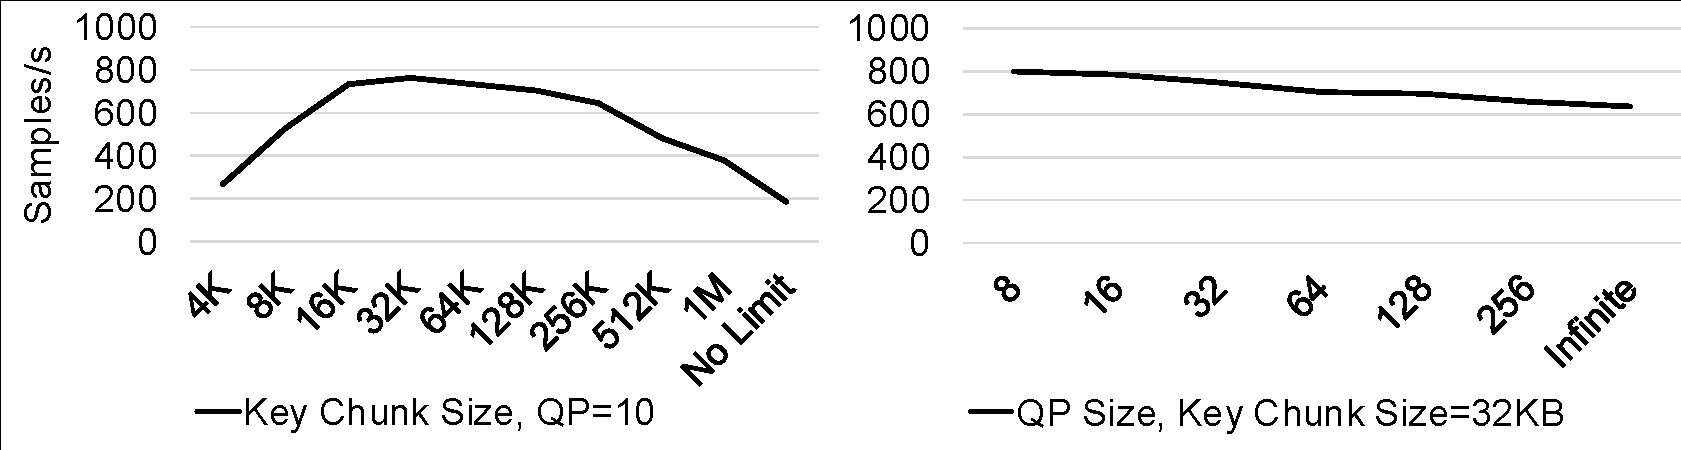
\includegraphics[width=.7\columnwidth,trim=4 8 2 4,clip,]{Figures/QPandKeyChunkSize.pdf}
	\caption{Effect of chunk size and queue pair count on throughput.}
	\label{fig:QPandKeyChunk}
\end{figure}

\vspace{0.05in}
\noindent \textbf{Size of key chunks:}
%\subsubsection{Size of key chunks}
\label{sec:keyChunking}
\phub leverages fine-grained key chunking to better balance load and overlap gradient reception and aggregation. Figure \ref{fig:QPandKeyChunk} (left) evaluates the effect of chunk size with \code{ZeroComputeEngine} on \pbox. Larger chunk sizes improved network utilization, while smaller sizes improved overlapping. We found 32KB chunk size to be optimum: this is likely due to our interfaces' maximum injection rate and aggregation pipeline latency.

\vspace{0.05in}
\noindent \textbf{Queue Pair Count:}
%\subsubsection{Queue Pair Count}
%\phub uses queue pairs to direct keys to cores. The card manages queue pairs; hence, 
A worker needs at least one queue pair per interface with which it communicates. Queue pairs have state, which is cached on the card. When that cache misses frequently, communication slows. For \pbox to use 10 interfaces, we need a minimum of 10 queue pairs per worker. More queue pairs could enable concurrent transmission from the same worker and reduce head of line blocking, but it increases the queue pair cache miss rate. Figure \ref{fig:QPandKeyChunk} (right) evaluates the tradeoff, showing that fewer queue pairs was optimal.





\subsection{Limits on Scalability}
\label{sec:scability} 
The scalability of \phub is inherently limited by available total memory, network or PCIe bandwidth. This section explores how close \phub gets to these limits. We use \pbox to answer these questions. \pbox achieves a 1:1 read:write memory bandwidth of 120 GB/s and a bidirectional network bandwidth of 140 GB/s. To determine how much bandwidth can be utilized,
%we configured varying numbers of worker machines running \code{ib\_write\_bw},
we added an additional IB interface to each of our 8 machines to emulate 16 workers and configured varying numbers of emulated workers running \code{ib\_write\_bw},
%, and configured varying numbers of worker machines running \code{ib\_write\_bw},
each with 10 QP connections to the \code{ib\_write\_bw} process on \pbox. These pairs of processes did repeated RDMA-writes to two 1 MB buffers on the other side. We set the PCIe read request size to 512 bytes. This configuration was chosen to mirror the setup of an actual training system while maximizing total system throughput. 
%We used \code{likwid} to measure the maximum system throughput in terms of memory bandwidth. 

To our surprise, we found that the peak memory bandwidth usage never exceeded more than 90 GB/s, far from the limit of both the aggregate network card and memory. This suggests that the bottleneck lies somewhere else. 

We then built a loopback microbenchmark that used the IB cards to copy data locally between RDMA buffers. This isolated the system from network bottlenecks and involved only the NIC's DMA controllers and the processor's PCIe-to-memory-system bridge. This microbenchmark also achieved only 90 GB/s. Based on this experiment, we believe that \textit{the limit of throughput in our current \phub system is the PCIe-to-memory-system bridge.}

\begin{figure}[t!]
    \centering
	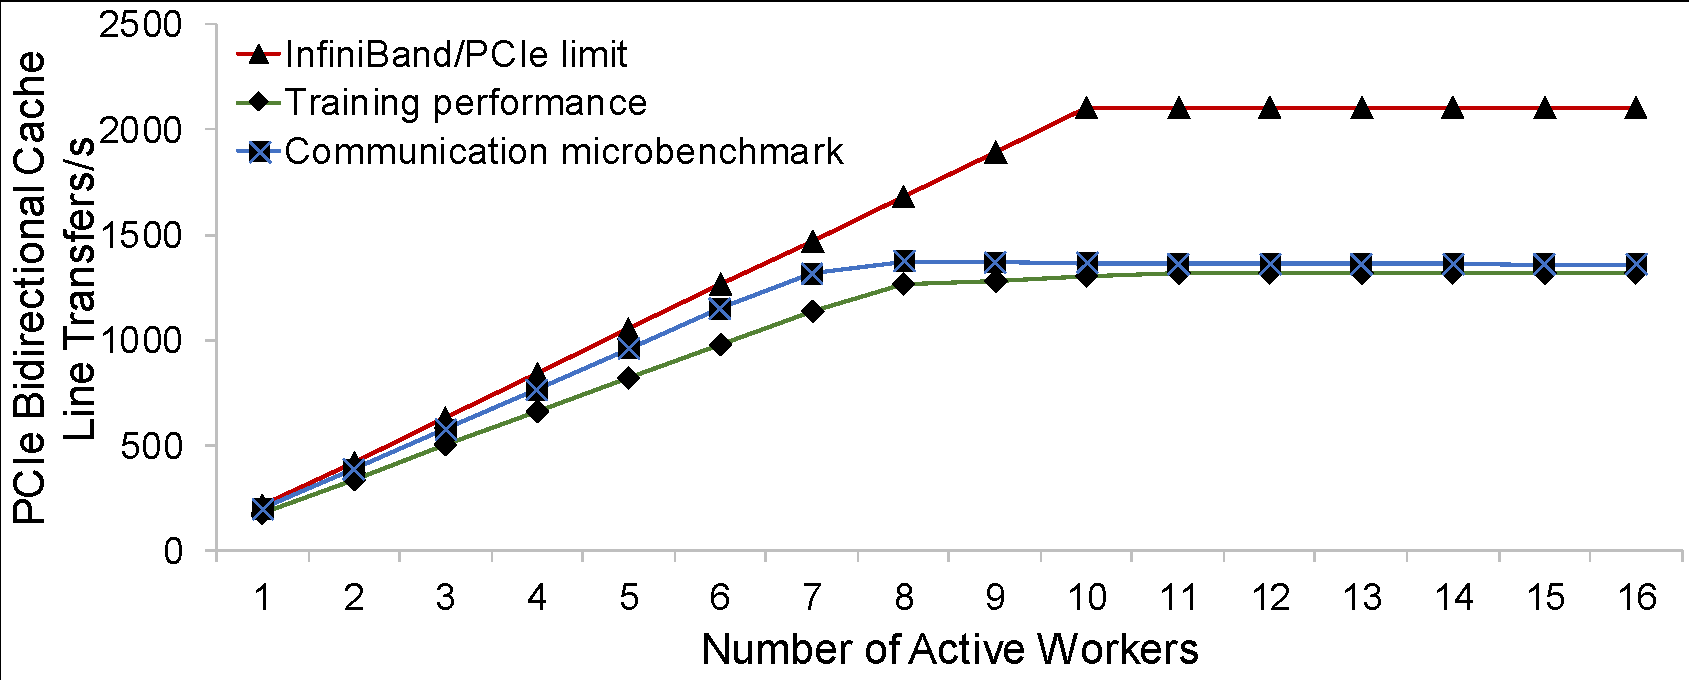
\includegraphics[width=.6\linewidth,trim=3 2 2 2,clip]{Figures/Scalability.pdf}
	\caption{\pbox{} scalability is limited by the throughput of the PCIe to the on-chip network bridge of the PBox processors. \phub{} can utilize 97\% of the measured peak PCIe bandwidth.}
	\label{fig:scalablity}
\end{figure}

Figure \ref{fig:scalablity} summarizes this experiment. The InfiniBand/PCIe limit line shows an ideal case where unlimited cache line transfers can be performed. However, this rate was not achievable even with a microbenchmark, which poses a hard upper bound on how fast \phub can run during training. We also see that, when training VGG with \code{ZeroComputeEngine}, as more workers are added, \pbox{}'s performance approached the microbenchmarks (97\%), demonstrating \phub{}'s ability to fully utilize system resources. The gap in the plot between \pbox and the microbenchmark %before they overlap 
is due to the overhead of scheduling operations in MxNet and straggler effects in workers. \pbox{} hit the limit at a sustained 80GB/s memory bandwidth.

In real training, however, \pbox{}'s scalability limit was difficult to reach. Recent work (\cite{keskar2016large, lecun1524efficient}) describes the difficulty of generalization with large batch sizes; it is not advantageous to blindly scale deep learning to a large number of workers without considering statistical efficiency~\cite{youspeeding, koliousiscrossbow}. One example \cite{ImageNetIn1Hour} reports that ResNet 50's statistical efficiency drops with aggregate batch sizes larger than 8192 on a system with 256 GPUs on 32 machines (with a mini-batch size of 32 per GPU). To assess whether \pbox could reach this scale, we measured the memory bandwidth usage for ResNet 50 with 8 workers using the same batch size. We found that \pbox required only 6GB/s memory bandwidth and an aggregated 4GB/s network bandwidth. This suggests that our \pbox prototype could scale to rack-level and support up to 120 worker machines training this network. In other words, our prototype could support sufficient scalability to handle cutting-edge training tasks.

On the other hand, the scalability bottleneck (PCIe controller) in our current prototype is specific to this particular platform, but it can change. For example, recently released AMD Epyc~\cite{AMDEpyc} processors provide nearly triple the Stream Triad performance
(290 GB/s)~\cite{EpycBenchmark} and 40\% more PCIe bandwidth than our
\pbox machine. We would expect Epyc to support 40\% more
throughput.
%Our test cluster does not have enough machines to saturate either of these, but we can project when scalability will stop based on these limits.


\subsection{Effectiveness of \pbox as a Rack-Scale Service}
\label{sec:hierarchicalEval}
We now evaluate effectiveness of \pbox as a rack-scale service with two typical scenarios in a 10 Gbps cloud-like environment: (1) when multiple jobs are training in parallel in a rack, sharing the same \pbox instance with different key namespaces and (2) when a training job crosses rack boundaries, and \phub performs hierarchical reduction.

\begin{figure}[t!]
    \centering
	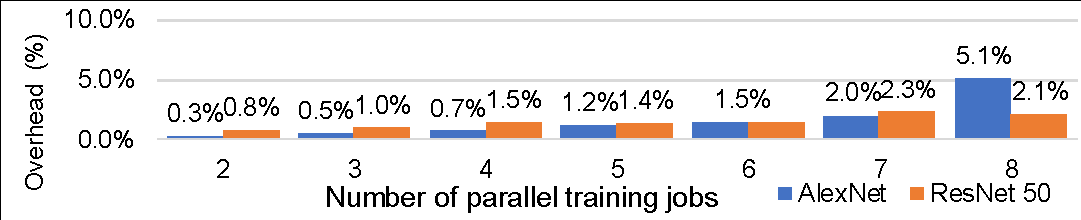
\includegraphics[width=.7\linewidth,trim=2 2 2 2,clip]{Figures/MultijobSim.pdf}
	\caption{Overhead of multiple parallel training jobs sharing the same \pbox instance.}
	\label{fig:multijobs}
\end{figure}

Figure \ref{fig:multijobs} shows the overhead of running multiple independent training jobs sharing a single \pbox. AlexNet saw a 5\% drop in per-job throughput when running 8 jobs, likely due to frequent invocation of optimizer and less effective caching; ResNet 50 saw a smaller impact as it is compute bound.

\begin{figure}[t!]
    \centering
	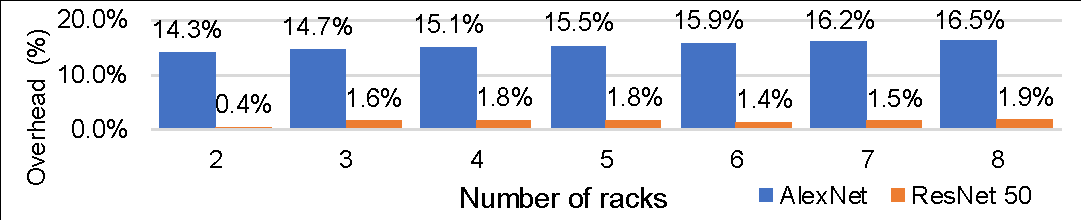
\includegraphics[width=.5\linewidth,trim=2 6 2 2,clip]{Figures/HierarchicalSim.pdf}
	\caption{Emulated overhead of hierarchical reduction with \pbox.}
	\label{fig:hierarchical}
\end{figure}

Figure \ref{fig:hierarchical} emulates a single cloud-based training job whose VMs span N racks, and each rack contains 8 workers and 1 \pbox. The \pbox uses a widely used ring reduction algorithm~\cite{baidures3:online,DBLP:journals/corr/abs-1802-05799} for inter-rack aggregation. 

Since we have only one \pbox machine, we model this ring reduction by sending and receiving N chunk-size messages sequentially, each performing one additional aggregation, for each of the keys, after local rack has finished aggregation. We assume each rack would finish its local aggregation at roughly the same time, as stragglers can exist regardless of rack assignment. Therefore, this faithfully estimates overhead of \phub{}'s hierarchical reduction.

AlexNet's throughput loss comes from added latency of multiple rounds of communication, but is compensated by drastically reduced cross-rack traffic, and thus we would expect speedup in real deployment. On the other hand, we again observed virtually no loss of throughput in ResNet 50.

\subsection{Rack-scale cost model}

Is a cluster built with PHubs and a slow network more cost effective than one with sharded PSs and a fast network? This section explores this question using a simple cost model. We consider the cost of three cluster components: worker nodes, PHub nodes, and network gear. We use advertised prices from the Internet; while a datacenter operator might pay less, the ratios between component prices should still be similar. The baseline is a cluster running MXNet IB with colocated sharded PSs; we compare this to a PHub deployment in terms of throughput per dollar.

The model works by computing the cost of a worker node, and adding to it the amortized cost of its network usage; for the PHub deployment, it also includes the amortized cost of the worker's PHub usage. This allows us to compare the cost of worker nodes in deployments with different numbers of workers per rack, switch, or PHub. We capture only the most significant cost, and include only capital cost, since operational costs are dominated by GPU power usage and thus differences would be small.

We model a standard three-layer datacenter network with some simplifying assumptions: racks hold as many machines as may be connected to a single switch, all switches and cables are identical, and oversubscription happens only at ToR switches. We model network costs by charging each worker the NIC per-port cost $N$, the amortized cost of one ToR switch port $S$ and cable $C$, and fractional costs of ToR/aggregation/core switch ports and cables depending on the oversubscription factor $F$. Thus, the amortized cost of the network per machine is $A=(N+S+C)+F(4S+2C)$. Since our goal is to model costs for future deployments, we make two changes from our experimental setup. Instead of 10Gb IB, we use 25 Gb Ethernet. Instead of NVIDIA 1080 Ti's, we assume a future GPU with similar cost $G$, but that performs like today's V100. This keeps the compute/communication ratio similar to that of our experiments. We use ResNet-50 for comparison; we use our 10Gb IB results for the PHub setting and downclocked 40Gb IB for the MXNet IB baseline. We include 2\% overhead in the PHub numbers to account for aggregation between racks.

%We use similar worker and PHub nodes as in our experiments. The cost $W$ is 

%% For the baseline, we use the same SuperMicro 1028GQ-TR worker nodes as in our evaluation, but with 4 GPUs. The advertised cost $W$ is \$4117~\cite{worker-price} without GPUs; we use the price of the NVIDIA GeForce 1080 Ti (\$699~\cite{nvidia-1080ti}) for the GPU price $G$. We use the Mellanox ConnectX-4 EN for 100Gb Ethernet (\$795~\cite{mellanox-eth}); the cost of a 2 meter cable is \$94~\cite{mellanox-cable}. The PHub worker nodes have the same configuration but with Mellanox ConnectX-4 Lx EN cards for 25Gb Ethernet (\$260~\cite{mellanox-eth}); the cable cost is \$31.25 using 4-to-1 breakout cables~\cite{mellanox-cable}. The PHub node is the same SuperMicro 6038R-TXR as in the evaluation; its cost $H$ is \$8407~\cite{phub-price}, and it uses 10 dual-port 25Gb Mellanox ConnectX-4 Lx EN cards (\$325~\cite{mellanox-eth}, or \$162.5 per port). We use the Arista 7060CX-32S 32-port 100Gb Ethernet switch (\$21077~\cite{}) in both configurations, with breakout cables to connect the 25Gb hosts. This means that with no oversubscription, a single switch can support 16 100Gb baseline workers, or a PHub and 44 25Gb workers. We assume 1 PHub per switch to allow for oversubscription; with 2:1 oversubscription each switch could support 65 25Gb workers; with 3:1 oversubscription, 76. The cost of each baseline worker is $W+N+4G+A$, and the cost of a PHub worker is $W+N+4G+A+KP$, where $KP$ is the amortized cost of the PHub ($P=W+20N$ and $K$ is the worker-to-phub ratio).

Workers are the same as in our evaluation, but with 4 GPUs. The cost $W$ is \$4117~\cite{worker-price} without GPUs; the GPU price $G$ is (\$699~\cite{nvidia-1080ti}). The 100Gb baseline uses Mellanox ConnectX-4 EN cards (\$795~\cite{mellanox-eth}) and 2m cables (\$94~\cite{mellanox-cable}). The 25Gb PHub workers use Mellanox ConnectX-4 Lx EN cards (\$260~\cite{mellanox-eth}) and 4-to-1 breakout cables (\$31.25 per port~\cite{mellanox-cable}).
The PHub node (also same as evaluation) cost $H$ is \$8407~\cite{phub-price}, plus 10 dual-port 25Gb Mellanox ConnectX-4 Lx EN cards (\$162.5 per port~\cite{mellanox-eth}). The cost of each baseline worker is $W+N+4G+A$, and the cost of a PHub worker is $W+N+4G+A+KP$, where $KP$ is the amortized PHub cost ($P=W+20N+20A$; $K$ is the worker to \phub ratio).

We use the Arista 7060CX-32S 32-port 100Gb Ethernet switch (\$21077~\cite{arista-price}) in both configurations, with breakout cables to connect 25Gb hosts.
With no oversubscription, each switch supports 16 100Gb baseline workers, or a PHub and 44 25Gb workers. With 2:1 oversubscription each switch could support a \phub and 65 25Gb workers; with 3:1, the number of supported workers is 76. 




%% \begin{table}[tb!]
%%   \centering
%%   \small
%%   \begin{tabular}{|r|c|c|c|}
%%     \hline
%%                   & Baseline         & PHub worker                & PHub \\
%%     \hline
%%     $W$ & \$4117~\cite{worker-price} & \$4117~\cite{worker-price} & \$8407~\cite{phub-price} \\
%%     $G$ & \$699~\cite{nvidia-1080ti} & \$699                      & \\
%%     $N$ & \$795~\cite{mellanox-eth}  & \$260                      & \$162.5/port \\
%%     $S$ & \$795~\cite{mellanox-eth}  & \$260                      & \$162.5/port \\
%%     \hline
%%   \end{tabular}
%%   \caption{Cost model parameters}
%%   \label{table:costModelParam}
%% \end{table}

\begin{table}[tb!]
  \centering
  \begin{tabular}{|r|c|c|c|}
    \hline
    & \multicolumn{3}{c|}{Throughput/\$1000} \\
    
                                 & Future GPUs & Spendy & Cheap \\
    \hline
    100Gb Sharded 1:1 &             46.11 &          14.57 &      60.41\\
    \hline 
    25Gb PHub     1:1 &             55.19 &          15.30 &      77.21\\
    \hline 
    25Gb PHub     2:1 &             57.71 &          15.49 &      82.24\\
    \hline 
    25Gb PHub     3:1 &             59.03 &          15.58 &      84.95\\
    \hline
  \end{tabular}
  \caption{Datacenter cost model comparing 25GbE PHub deployments with 100GbE MXNet IB on ResNet-50. Higher is better. The Future GPU PHub deployment with 2:1 oversubscription provides 25\% better throughput per dollar.}
  \label{table:costModel}
\end{table}

%% Table~\ref{table:costModel} compares a full-bisection-bandwidth 100GbE sharded MXNet IB deployment with 25GbE PHub deployments with varying oversubscription. With 2:1 oversubscription, the PHub deployment provides 26\% better throughput per dollar. We consider two other configurations. First, one using today's expensive V100s, where the 2:1 PHub deployment provides only 6\% better throughput per dollar: future GPUs this expensive are likely to be faster than this, so this configuration essentially provides a lower bound to improvement. Second, one using cheap (E5-2603 v4) in workers, providing 38\% better throughput per dollar: since the majority of training is done on the GPUs, CPU performance may not be important.

Table~\ref{table:costModel} compares a full-bisection-bandwidth 100GbE sharded MXNet IB deployment with 25GbE PHub deployments with varying oversubscription. With 2:1 oversubscription, the PHub deployment provides 26\% better throughput per dollar. We consider two other configurations: a ``lower bound'' using today's expensive V100's, where the 2:1 PHub deployment provides only 6\% improvement; and a ``GPU-focused'' one using cheap CPUs (E5-2603 v4) in workers, providing 36\% improvement.




